\section{Results}
\label{sec:results}

We compare four methods: \textbf{Random} (shuffle users into open tables, the ``seating chart drawn by a cat''), \textbf{Greedy} (repeatedly open the best table per seat), \textbf{Model A} (HiGHS on the compact MILP), and \textbf{Model B} (column generation). All runs use one CPU thread. Quality is measured against the certified upper bound~\eqref{eq:ub}, so a gap of $0\%$ means provably optimal.

\subsection{Quality: Model B is near-optimal, and provably so}

\begin{table}[h]
\centering\small
\begin{tabular}{@{}r rrrr rr@{}}
\toprule
& \multicolumn{4}{c}{Gap to upper bound (\%)} & \multicolumn{2}{c}{Seconds} \\
\cmidrule(lr){2-5}\cmidrule(l){6-7}
$N$ & Random & Greedy & Model A & Model B & Model A & Model B \\
\midrule
12 & 94.7 & 38.1 & 0.7 & 0.7 & 10.6 & 1.8 \\
18 & 106.9 & 23.2 & 0.9 & 1.2 & 26.8 & 4.8 \\
24 & 76.0 & 24.1 & 2.1 & 0.8 & 90.2 & 9.7 \\
30 & 78.0 & 19.9 & 8.7 & 0.9 & 90.3 & 41.6 \\
\bottomrule
\end{tabular}
\caption{Small instances. Model A gets a 90-second limit per instance. For $N\le 18$ it finishes, and Model B matches its proven optimum in 9 of 10 instances. For $N\ge 24$ Model A hits the time limit every time, while Model B stays within about 1\% of the bound in seconds.}
\label{tab:e1}
\end{table}

Table~\ref{tab:e1} and Figure~\ref{fig:qsc}a tell a consistent story. Random seating is not just bad but often \emph{negative}: it strands people who cannot make the slot it picked and seats others an hour from home. Greedy is far better but myopic. It fills the most attractive tables first and leaves 6--13\% of users with no feasible table at the end (Model B seats everyone in 19 of 20 instances). Model A is exact when it finishes, and it is the reason we trust the comparison: on the ten instances with $N\le18$, Model B equals Model A's proven optimum nine times and is 2\% short once. That one miss is the price of solving the final IP only over generated columns (``price-and-branch'') rather than generating columns inside every branch-and-bound node. From $N=24$ on, Model A runs out of time with gaps up to 13\%, while Model B finishes in 5--40 seconds and never exceeds a 1.9\% gap.

\subsection{Scale: the compact MILP stalls, column generation does not}

\begin{figure}[t]
\centering
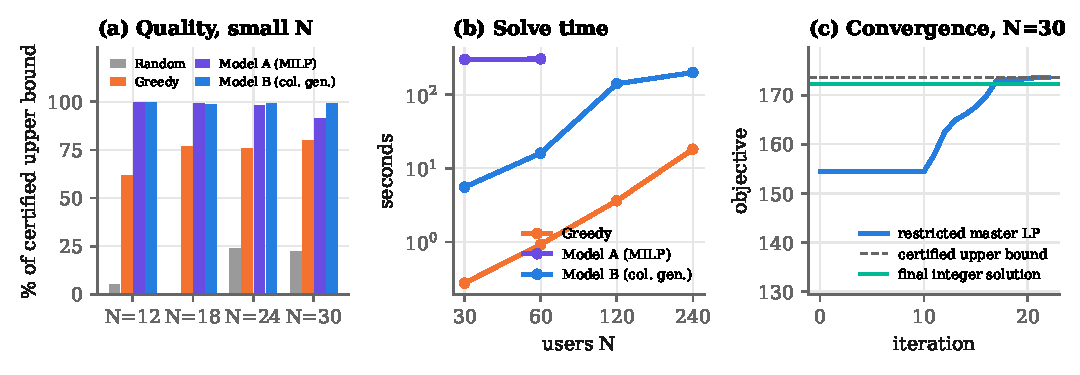
\includegraphics[width=\textwidth]{fig/quality_scale_cg.pdf}
\vspace{-14pt}
\caption{(a) Share of the certified upper bound achieved, averaged over 5 instances per $N$ (Random averages between $-7\%$ and $24\%$; a negative average is drawn at 0). (b) Mean solve time; Model A is stopped at 300 seconds. (c) One run of column generation at $N=30$: the restricted master LP climbs to the full LP optimum in 22 iterations using 312 of the roughly 350{,}000 possible tables, and exact pricing then certifies it as an upper bound.}
\label{fig:qsc}
\end{figure}

Figure~\ref{fig:qsc}b shows solve times up to $N=240$. Model A has $O(N^2|\K|)$ pair variables, over 5{,}000 variables in total at $N=30$, and its LP relaxation gives branch and bound little to prune with. At $N=60$, after 300 seconds, its best seating is worth only about 76\% of Model B's, which Model B finds in about 15 seconds. Model B's time grows because both the number of $(v,t)$ pairs and the pricing pool grow with $N$, but it still seats 240 users in about 3.5 minutes and beats Greedy by 9.5\% on average across $N\ge60$. The advantage shrinks with size, from 8--18\% at $N=60$ to 5--6\% at $N=240$, and Model B's own gap to its LP value grows from under 1\% to about 4\%. At that size our integer step (pool IP plus diving) becomes the bottleneck, which is the first thing full branch-and-price would fix.

Figure~\ref{fig:qsc}c shows column generation at work. The first restricted master contains only the greedy tables. Each round of pricing uses the duals $\pi_i$ and $\mu_{vt}$ to find tables with positive reduced cost~\eqref{eq:redcost}. The LP value rises quickly and then flattens. Exact pricing then finds no improving column, so the LP value \emph{is} the bound, and the integer solution is within 0.75\% of it.

\subsection{What the add-ons buy}

\begin{figure}[t]
\centering
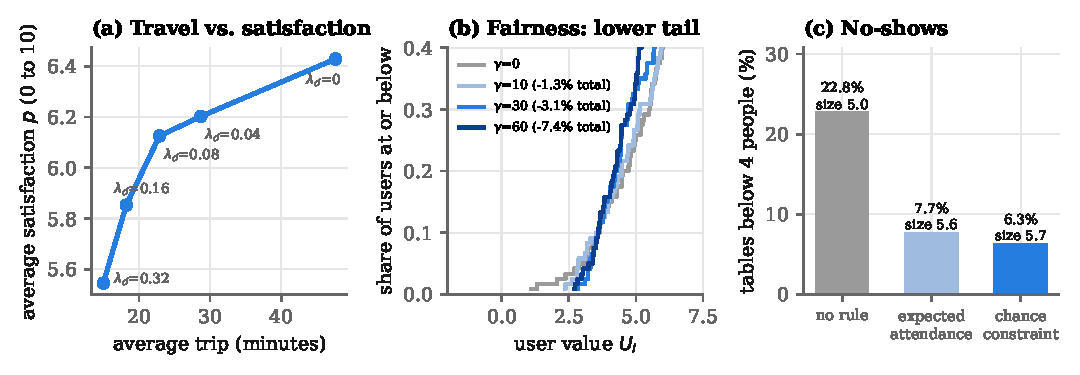
\includegraphics[width=\textwidth]{fig/tradeoffs.pdf}
\vspace{-14pt}
\caption{Trade-offs at $N=60$ (Model B). (a) Raising the value of time $\lambda_d$ shortens trips much faster than it lowers satisfaction, until $\lambda_d=0.32$. (b) Distribution of user value $U_i$, lower tail only: the fairness floor lifts the worst-off users from about $-0.5$ to about $4$ for a 1--3\% drop in total value. (c) Share of tables that drop below four people in 5{,}000 simulated evenings, with the average table size above each bar.}
\label{fig:trade}
\end{figure}

\paragraph{Travel.} In Figure~\ref{fig:trade}a, moving from $\lambda_d=0$ (travel is free) to our default $\lambda_d=0.08$ cuts the average trip from 50 to 23 minutes, a 54\% drop, while average satisfaction $p$ falls only from 6.29 to 6.00 out of 10. The share of users paying a bridge toll falls from 5\% to under 1\%. The curve bends sharply after $\lambda_d=0.16$: squeezing trips below 19 minutes starts sending people to places they do not like. This is the shadow-price way to read $\lambda_d$: it is the exchange rate between a minute and a point of satisfaction, and the knee tells us where the exchange gets expensive.

\paragraph{Fairness.} With $\gamma=0$ the solver happily gives a few users a value near zero to help everyone else. A modest weight $\gamma=10$ raises the worst user's value $\theta$ from $-0.45$ to $3.9$ on average and costs only 1.2\% of total value (Figure~\ref{fig:trade}b). Larger $\gamma$ buys little extra floor for more cost. In the reduced cost this appears as the reweighting $(1+\sigma_i)$: users with a positive fairness dual $\sigma_i$ become more valuable to seat well.

\paragraph{No-shows.} With no rule, 15.3\% of tables lose enough people to fall below four (Figure~\ref{fig:trade}c). The linear proxy in Model A, expected attendance $\sum_i\phi_i x_{ik}\ge 4.25$, cuts this to 5.7\%. The exact chance constraint with $\alpha=0.9$, available only in Model B, cuts it to 4.2\% and guarantees that \emph{every} table's risk is below 10\%, which the proxy cannot promise (on one instance the proxy's tables averaged an 8.4\% risk). Both rules work mostly by making tables bigger, and they cost about 1.0\% and 1.5\% of planned value.

\section{Discussion}
\label{sec:discussion}

\paragraph{What worked and why.} Column generation wins for two reasons. First, the set partitioning LP is much tighter than Model A's LP: in Model A a fractional user can be ``a sixth at every table,'' while in Model B the LP can only mix whole, sensible tables. A tighter relaxation means better bounds, which is exactly what branch and bound needs. Second, every table-level rule, including the pairs, the age range, and the nonlinear chance constraint, becomes a number computed once per column instead of new variables and big-$M$ constraints. Duals and reduced costs, which in class we used mainly to read sensitivity off a final tableau, here drive the whole algorithm.

\paragraph{Limitations.} (1) Our integer step is price-and-branch, not full branch-and-price, so Model B is not guaranteed optimal; it was 2\% short in one small case. (2) Exact pricing is a quadratic knapsack MILP, and beyond about 30 users it is too slow to run to completion, so for large $N$ we report the gap to the LP value under heuristic pricing, which is not a certified bound. (3) The data are synthetic, and the travel model (a fixed detour factor, a constant speed, and one bridge) is crude. (4) No-shows are assumed independent; friends who cancel together would break that.

\paragraph{Next steps.} The obvious next step is a short survey of real users to replace the generator; the model needs no change, only new values of $p_{ivt}$ and $q_{ij}$. On the methods side, branching on pairs (``$i$ and $j$ together or apart,'' the Ryan--Foster rule) would turn price-and-branch into exact branch-and-price. Finally, a weekly version could set $q_{ij}=-\infty$ for pairs who have already met, so the city keeps getting a little smaller. After that, \emph{Table for 6} becomes a product: we already have a Streamlit and HiGHS stack from our first prototype, and the solver is fast enough to run while someone waits for their coffee.
